\documentclass[
  shownotes,
  xcolor={svgnames},
  hyperref={colorlinks,citecolor=DarkBlue,linkcolor=DarkRed,urlcolor=DarkBlue}
  , aspectratio=169]{beamer}
\usepackage{animate}
\usepackage{amsmath}
\usepackage{amsfonts}
\usepackage{amssymb}
\usepackage{pifont}
\usepackage{mathpazo}
%\usepackage{xcolor}
\usepackage{multimedia}
\usepackage{fancybox}
\usepackage[para]{threeparttable}
\usepackage{multirow}
\setcounter{MaxMatrixCols}{30}
\usepackage{subcaption}
\usepackage{graphicx}
\usepackage{lscape}
\usepackage[compatibility=false,font=small]{caption}
\usepackage{booktabs}
\usepackage{ragged2e}
\usepackage{chronosys}
\usepackage{appendixnumberbeamer}
\usepackage{animate}
\setbeamertemplate{caption}[numbered]
\usepackage{color}
%\usepackage{times}
\usepackage{tikz}
\usepackage{comment} %to comment
%% BibTeX settings
\usepackage{natbib}
\bibliographystyle{apalike}
\bibpunct{(}{)}{,}{a}{,}{,}
\setbeamertemplate{bibliography item}{[\theenumiv]}

% Defines columns for bespoke tables
\usepackage{array}
\newcolumntype{L}[1]{>{\raggedright\let\newline\\\arraybackslash\hspace{0pt}}m{#1}}
\newcolumntype{C}[1]{>{\centering\let\newline\\\arraybackslash\hspace{0pt}}m{#1}}
\newcolumntype{R}[1]{>{\raggedleft\let\newline\\\arraybackslash\hspace{0pt}}m{#1}}


\usepackage{xfrac}


\usepackage{multicol}
\setlength{\columnsep}{0.5cm}

% Theme and colors
\usetheme{Boadilla}

% I use steel blue and a custom color palette. This defines it.
\definecolor{andesred}{HTML}{af2433}

% Other options
\providecommand{\U}[1]{\protect\rule{.1in}{.1in}}
\usefonttheme{serif}
\setbeamertemplate{itemize items}[default]
\setbeamertemplate{enumerate items}[square]
\setbeamertemplate{section in toc}[circle]

\makeatletter

\definecolor{mybackground}{HTML}{82CAFA}
\definecolor{myforeground}{HTML}{0000A0}

\setbeamercolor{normal text}{fg=black,bg=white}
\setbeamercolor{alerted text}{fg=red}
\setbeamercolor{example text}{fg=black}

\setbeamercolor{background canvas}{fg=myforeground, bg=white}
\setbeamercolor{background}{fg=myforeground, bg=mybackground}

\setbeamercolor{palette primary}{fg=black, bg=gray!30!white}
\setbeamercolor{palette secondary}{fg=black, bg=gray!20!white}
\setbeamercolor{palette tertiary}{fg=white, bg=andesred}

\setbeamercolor{frametitle}{fg=andesred}
\setbeamercolor{title}{fg=andesred}
\setbeamercolor{block title}{fg=andesred}
\setbeamercolor{itemize item}{fg=andesred}
\setbeamercolor{itemize subitem}{fg=andesred}
\setbeamercolor{itemize subsubitem}{fg=andesred}
\setbeamercolor{enumerate item}{fg=andesred}
\setbeamercolor{item projected}{bg=gray!30!white,fg=andesred}
\setbeamercolor{enumerate subitem}{fg=andesred}
\setbeamercolor{section number projected}{bg=gray!30!white,fg=andesred}
\setbeamercolor{section in toc}{fg=andesred}
\setbeamercolor{caption name}{fg=andesred}
\setbeamercolor{button}{bg=gray!30!white,fg=andesred}


\usepackage{fancyvrb}
\newcommand{\VerbBar}{|}
\newcommand{\VERB}{\Verb[commandchars=\\\{\}]}
\DefineVerbatimEnvironment{Highlighting}{Verbatim}{commandchars=\\\{\}}
% Add ',fontsize=\small' for more characters per line
\usepackage{framed}
\definecolor{shadecolor}{RGB}{248,248,248}
\newenvironment{Shaded}{\begin{snugshade}}{\end{snugshade}}
\newcommand{\AlertTok}[1]{\textcolor[rgb]{0.94,0.16,0.16}{#1}}
\newcommand{\AnnotationTok}[1]{\textcolor[rgb]{0.56,0.35,0.01}{\textbf{\textit{#1}}}}
\newcommand{\AttributeTok}[1]{\textcolor[rgb]{0.77,0.63,0.00}{#1}}
\newcommand{\BaseNTok}[1]{\textcolor[rgb]{0.00,0.00,0.81}{#1}}
\newcommand{\BuiltInTok}[1]{#1}
\newcommand{\CharTok}[1]{\textcolor[rgb]{0.31,0.60,0.02}{#1}}
\newcommand{\CommentTok}[1]{\textcolor[rgb]{0.56,0.35,0.01}{\textit{#1}}}
\newcommand{\CommentVarTok}[1]{\textcolor[rgb]{0.56,0.35,0.01}{\textbf{\textit{#1}}}}
\newcommand{\ConstantTok}[1]{\textcolor[rgb]{0.00,0.00,0.00}{#1}}
\newcommand{\ControlFlowTok}[1]{\textcolor[rgb]{0.13,0.29,0.53}{\textbf{#1}}}
\newcommand{\DataTypeTok}[1]{\textcolor[rgb]{0.13,0.29,0.53}{#1}}
\newcommand{\DecValTok}[1]{\textcolor[rgb]{0.00,0.00,0.81}{#1}}
\newcommand{\DocumentationTok}[1]{\textcolor[rgb]{0.56,0.35,0.01}{\textbf{\textit{#1}}}}
\newcommand{\ErrorTok}[1]{\textcolor[rgb]{0.64,0.00,0.00}{\textbf{#1}}}
\newcommand{\ExtensionTok}[1]{#1}
\newcommand{\FloatTok}[1]{\textcolor[rgb]{0.00,0.00,0.81}{#1}}
\newcommand{\FunctionTok}[1]{\textcolor[rgb]{0.00,0.00,0.00}{#1}}
\newcommand{\ImportTok}[1]{#1}
\newcommand{\InformationTok}[1]{\textcolor[rgb]{0.56,0.35,0.01}{\textbf{\textit{#1}}}}
\newcommand{\KeywordTok}[1]{\textcolor[rgb]{0.13,0.29,0.53}{\textbf{#1}}}
\newcommand{\NormalTok}[1]{#1}
\newcommand{\OperatorTok}[1]{\textcolor[rgb]{0.81,0.36,0.00}{\textbf{#1}}}
\newcommand{\OtherTok}[1]{\textcolor[rgb]{0.56,0.35,0.01}{#1}}
\newcommand{\PreprocessorTok}[1]{\textcolor[rgb]{0.56,0.35,0.01}{\textit{#1}}}
\newcommand{\RegionMarkerTok}[1]{#1}
\newcommand{\SpecialCharTok}[1]{\textcolor[rgb]{0.00,0.00,0.00}{#1}}
\newcommand{\SpecialStringTok}[1]{\textcolor[rgb]{0.31,0.60,0.02}{#1}}
\newcommand{\StringTok}[1]{\textcolor[rgb]{0.31,0.60,0.02}{#1}}
\newcommand{\VariableTok}[1]{\textcolor[rgb]{0.00,0.00,0.00}{#1}}
\newcommand{\VerbatimStringTok}[1]{\textcolor[rgb]{0.31,0.60,0.02}{#1}}
\newcommand{\WarningTok}[1]{\textcolor[rgb]{0.56,0.35,0.01}{\textbf{\textit{#1}}}}
\usepackage{graphicx}
\makeatletter


% colors
\definecolor{airforceblue}{rgb}{0.36, 0.54, 0.66}
\newcommand{\theme}{\color{andesred}}
\newcommand{\bk}{\color{black}}
\newcommand{\rd}{\color{red}}
\newcommand{\fg}{\color{ForestGreen}}
\newcommand{\bl}{\color{blue}}
\newcommand{\gr}{\color{black!60}}
\newcommand{\sg}{\color{DarkSlateGray}}
\newcommand{\br}{\color{SaddleBrown}}
\newcommand{\nv}{\color{Navy}}


% common math markups
\newcommand{\bs}[1]{\boldsymbol{#1}}
\newcommand{\mc}[1]{\mathcal{#1}}
\newcommand{\mr}[1]{\mathrm{#1}}
\newcommand{\bm}[1]{\mathbf{#1}}
\newcommand{\ds}[1]{\mathds{#1}}
\newcommand{\indep}{\perp\!\!\!\perp}



% shorthand
\newcommand{\sk}{\vspace{.5cm}}
\newcommand{\R}[1]{{\tt \nv #1}}
\newcommand{\til}{{\footnotesize$\bs{\stackrel{\sim}{}}$}}
\DeclareSymbolFont{extraup}{U}{zavm}{m}{n}
\DeclareMathSymbol{\vardiamond}{\mathalpha}{extraup}{87}

\usepackage{tikz}
% Tikz settings optimized for causal graphs.
\usetikzlibrary{shapes,decorations,arrows,calc,arrows.meta,fit,positioning}
\tikzset{
    -Latex,auto,node distance =1 cm and 1 cm,semithick,
    state/.style ={ellipse, draw, minimum width = 0.7 cm},
    point/.style = {circle, draw, inner sep=0.04cm,fill,node contents={}},
    bidirected/.style={Latex-Latex,dashed},
    el/.style = {inner sep=2pt, align=left, sloped}
}


\makeatother





%%%%%%%%%%%%%%% BEGINS DOCUMENT %%%%%%%%%%%%%%%%%%

\begin{document}

\title[Lecture 26]{Lecture 26: \\ PCA (cont.) }
\subtitle{Big Data and Machine Learning for Applied Economics \\ Econ 4676}
\date{\today}

\author[Sarmiento-Barbieri]{Ignacio Sarmiento-Barbieri}
\institute[Uniandes]{Universidad de los Andes}


\begin{frame}[noframenumbering]
\maketitle
\end{frame}

%%%%%%%%%%%%%%%%%%%%%%%%%%%%%%%%%%%


%%%%%%%%%%%%%%%%%%%%%%%%%%%%%%%%%%%



%----------------------------------------------------------------------% 

\begin{frame}
\frametitle{Agenda}

\tableofcontents

\end{frame}

%----------------------------------------------------------------------%
\section{Factor Models}
%----------------------------------------------------------------------%


\begin{frame}
\frametitle{Factor Models}

\begin{itemize}
\item Text is super high dimensional
\medskip
\item There is often abundant {\it unlabeled} text
\medskip
\item Some times unsupervized factor model is a popular and useful strategy with text data
\medskip
\item You can first fit a factor model to a giant corpus, get a few factors (reduce the dimensionality)
\medskip
\item Use these factors for supervised learning on a subset of labeled documents.
\medskip
\item The unsupervised dimension reduction facilitates the supervised learning
\end{itemize}
\end{frame}


%----------------------------------------------------------------------%
\begin{frame}
\frametitle{Topic Models: Example}

\begin{itemize}


\item We have 6,166 reviews, with an average length of 90 words per review, \url{we8there.com}. 
\medskip
\item A useful feature of these reviews is that they contain both text and a multidimensional rating on overall experience, atmosphere, food, service, and value. 
\medskip
\item For example, one user submitted a glowing review for Waffle House \#1258 in Bossier City, Louisiana: 
\medskip

\begin{quote}
I normally would not revue a Waffle House but this one deserves it. The workers, Amanda, Amy, Cherry, James and J.D. were the most pleasant crew I have seen. While it was only lunch, B.L.T. and chili, it was great. The best thing was the 50’ s rock and roll music, not to loud not to soft. This is a rare exception to what you all think a Waffle House is. Keep up the good work. \\
Overall: 5, Atmosphere: 5, Food: 5, Service: 5, Value: 5.  
 \end{quote} 


\end{itemize}
\end{frame}
%----------------------------------------------------------------------%
\begin{frame}[fragile]
\frametitle{Topic Models: Example}


\begin{itemize}


\item We can apply PCA to get a factor representation of the review text. 
\item  PC1 looks like it will be big and positive for positive reviews, 

\begin{scriptsize}

\begin{Shaded}
\begin{Highlighting}[]
\NormalTok{pca \textless{}{-}}\StringTok{ }\KeywordTok{prcomp}\NormalTok{(x, }\DataTypeTok{scale=}\OtherTok{TRUE}\NormalTok{) }\CommentTok{\# can take a long time}

\KeywordTok{tail}\NormalTok{(}\KeywordTok{sort}\NormalTok{(pca}\OperatorTok{$}\NormalTok{rotation[,}\DecValTok{1}\NormalTok{]))}
\end{Highlighting}
\end{Shaded}

\end{scriptsize}
\begin{tiny}

\begin{verbatim}
##     food great     staff veri     excel food high recommend     great food 
##    0.007386860    0.007593374    0.007629771    0.007821171    0.008503594 
##     food excel 
##    0.008736181
\end{verbatim}

\end{tiny}
\medskip



\item while PC4 will be big and negative 
\begin{scriptsize}
\begin{Shaded}
\begin{Highlighting}[]
\KeywordTok{tail}\NormalTok{(}\KeywordTok{sort}\NormalTok{(pca}\OperatorTok{$}\NormalTok{rotation[,}\DecValTok{4}\NormalTok{]))}
\end{Highlighting}
\end{Shaded}
\end{scriptsize}
\begin{tiny}

\begin{verbatim}
##   order got after minut  never came   ask check readi order drink order 
##  0.05918712  0.05958572  0.06099509  0.06184512  0.06776281  0.07980788
\end{verbatim}
\end{tiny}




\end{itemize}
\end{frame}


%----------------------------------------------------------------------%
\begin{frame}
\frametitle{Factor Models}

\begin{itemize}
  \item Lets assume that we have a data matrix $X_{n\times p}$
  \medskip
\item A factor model looks like 

\begin{align}
X_{1}&=  \phi_{11} f_{1} + \dots + \phi_{1k} f_{k} \\ \nonumber
X_{2}&=  \phi_{21} f_{1} + \dots + \phi_{2k} f_{k} \\ \nonumber
&\vdots  \\ \nonumber
X_{p} &=  \phi_{p1} f_{1} + \dots + \phi_{pk} f_{k} \\ \nonumber
\end{align}

\item where 
  \begin{itemize}
    \footnotesize
   \item $X_{j}$ are the inputs of the regressions (independent vars)
   \medskip
   \item The $f_{k}$ $k=1,\dots K$ are the factors, unobserved, and that we want to estimate
  \medskip
   \item $\phi_{jk}$  are called loadings or rotations—these
  \medskip
   \item When you use a $K$ that is much smaller than $p$, factor models provide a parsimonious representation for $X$. 
   
  \end{itemize}


\end{itemize}
\end{frame}
%----------------------------------------------------------------------%
\begin{frame}
\frametitle{Factor Models: PCA}

\begin{itemize}
\item How do you estimate a Factor Model with PCA?
\medskip
\item We are trying to learn from high-dimensional $X$ some low-dimensional summaries that contain the information necessary to make good decisions. 
\pause
\medskip
\item Suppose that there is only one underlying factor $f_1$
\medskip

\begin{align}
x_{1}&=  \phi_{11} f_{1} \\ \nonumber
x_{2}&=  \phi_{21} f_{1} \\ \nonumber
&\vdots  \\ \nonumber
x_{p} &=  \phi_{p1} f_{1} \\ \nonumber
\end{align}


\end{itemize}
\end{frame}
%----------------------------------------------------------------------%
\begin{frame}
\frametitle{Factor Models: PCA}

\begin{itemize}

\item or in a more compact form form
\begin{align}
X = \phi_1 f_1
\end{align}

\item and

\begin{align}
f_1 = \phi_1^{-1}X
\end{align}

\item so we don't have to deal with inverses (things do not change), let's call $\delta_1=\phi_1^{-1}$

\begin{align}
f_1 = \delta_1 X
\end{align}
\end{itemize}


\end{frame}
%----------------------------------------------------------------------%
\begin{frame}
\frametitle{Detour: Algebra Review}

\begin{itemize}

\item Let $A_{m\times m}$. It exists 
\begin{itemize}
  \item a scalar $\lambda$ such that $Ap = \lambda p$ for a vector $p_{m\times 1}$, 
  \item if $p \neq 0$, then $\lambda$ is an eigenvalue of A. 
  \item and $p$ is an eigenvector of A corresponding to the eigenvalue $\lambda$.
\end{itemize}

\item $A_{m\times m}$ with eigenvalues $\lambda_1, \lambda_2,\dots,\lambda_m$, then:

\begin{align}
tr(A) &= \sum_{i=1}^m \lambda_i \\
det(A) &= \Pi_{i=1}^m \lambda_i
\end{align}

\item If $A_{m\times m}$ has $m$ different eigenvalues, then the associated eigenvectors are all linearly independent.
\end{itemize}
\end{frame}
%----------------------------------------------------------------------%
\begin{frame}
\frametitle{Detour: Algebra Review}
\begin{itemize}
\item Spectral decomposition: 
\medskip
\begin{align}
A = P\Lambda P
\end{align}
 
\item where $\Lambda = diag(\lambda_1, \dots \lambda_m )$ and $P$ is the matrix whose columns are the corresponding eigenvectors.
\end{itemize}
\begin{align}
A=\left(\begin{array}{ccccc}
p_{1} & p_{2} & \dots & \dots & p_{m}\end{array}\right)\left(\begin{array}{ccccc}
\lambda_{1} &  &  &  & 0\\
 & \lambda_{2}\\
 &  & \ddots\\
 &  &  & \ddots\\
0 &  &  &  & \lambda_{m}
\end{array}\right)\left(\begin{array}{c}
p_{1}\\
p_{2}\\
\vdots\\
\vdots\\
p_{m}
\end{array}\right)
\end{align}
\begin{align}
A=\sum_{i=1}^{m}\lambda_{i}p_{i}p_{i}'
\end{align}

\end{frame}

%----------------------------------------------------------------------%
\section{PCA: Theory}
%----------------------------------------------------------------------%
\begin{frame}
\frametitle{Principal Component Analysis}

\begin{align}
f_1 = \delta_1 X
\end{align}


\begin{itemize}

  \item The task is then finding the best linear combination of the original variables.
  \medskip
  \item What is best?
  \medskip
  \pause
  \item PCA response: the one that preserves the most information
  \medskip
  \item In other words, we are going to try to generate an index that reproduces (the best it can) the information (variability) of the original variables
  \medskip
  \item How we do that?
  \pause
  \medskip
  \item Maximize the variance

\end{itemize}   
\end{frame}
%----------------------------------------------------------------------%
\begin{frame}
\frametitle{Principal Component Analysis}

\begin{itemize}
  \item The problem then looks like

  \begin{align}
  max V(f_1) = max V(\delta_1 X)
  \end{align}

  \item where
  \begin{itemize}
    \item $X = (x_1 , \dots , x_K)_{N \times K}$  , 
    \item $S = V(X)$ 
    \item $\delta_1 \in K$
 \end{itemize}
  \item Let's set up the problem as 
  \begin{align}
  \underset{\delta}{max}\,\,\, \delta_1 X \delta'_1
  \end{align}

  \item What is the solution to this problem?

 \pause
  \item Bring $\delta$ to infinity. 
 
\end{itemize}
 \end{frame}


%----------------------------------------------------------------------%
\begin{frame}
\frametitle{Principal Component Analysis}

\begin{itemize}
\item Let's "fix" the problem by normalizing $\delta$

\begin{align}
\underset{\delta}{max}\,\, \delta_1 S \delta'_1 \\ \nonumber
\text{subject to}  \\ \nonumber
\delta_1 \delta'_1 = 1 \nonumber
\end{align}
\item Let us call the solution to this problem $\delta^*_1$. 
\medskip
\item $f^*_1 = \delta^*_1 X$ is the 'best' linear combination of X. 
\medskip
\item Intuition: $X$ has $K$ columns and $f^*_1 = \delta^*_1 X$ has only one. The factor built with the first principal component is the best way to represent the K variables of X using a single single variable.
\end{itemize}
\end{frame}


%----------------------------------------------------------------------%
\begin{frame}
\frametitle{Principal Component Analysis}

\begin{itemize}


\item Solution to the problem of the first principal component

\medskip
\item Let's set the lagrangian
\begin{align}
\mathcal{L} = \delta_1 S \delta'_1 + \lambda_1 (1-\delta_1\delta'_1)
\end{align}


\item Rearranging

\begin{align}
S \delta'_1 = \lambda_1 \delta'_1
\end{align}

 \item At the optimum, $\delta$ is the eigenvector corresponding to the eigenvalue $\lambda$ of $S$. 

\item Premultiplying by $\delta_1$ and  remembering that $\delta_1\delta'_1=1$:

\end{itemize}
\end{frame}


%----------------------------------------------------------------------%
\begin{frame}
\frametitle{Principal Component Analysis}




\begin{align}
\delta_1 S \delta'_1 = \lambda_1 
\end{align}
\begin{itemize}
\item In order to maximize $\delta S \delta $ we must choose $\lambda$ equal to the maximum eigenvalue of $S$ and $\delta$ is the corresponding eigenvalue.
\medskip
\item The problem of finding the best linear combination that reproduces the variability of $X$ is finding the biggest eigenvalue of $S$ and it's corresponding eigenvector

\end{itemize}
\end{frame}

%----------------------------------------------------------------------%
\begin{frame}
\frametitle{Principal Component Analysis}

\begin{itemize}

\item The first main component? Are there others?

\item Let's consider the following problem:
\begin{align}
\underset{\delta_2}{max}\,\, \delta_2 S \delta'_2 \\
\text{st}   \\
\delta_2 \delta'_2 &= 1   \\
\delta_2 \delta'_1 &=0 \\ \nonumber
\end{align}

\item $f_2^*=\delta^*_2X$ is the second principal component : the best linear combination which is
orthogonal to the best initial linear combination.
\item Recursively, using this logic you can form q  main components. 
\item Note that algebraically we could construct $q = K$ factors, actually the number of PC are $min(n-1,K)$ 
\end{itemize}

\end{frame}

%----------------------------------------------------------------------%
\begin{frame}
\frametitle{q main components}

\begin{itemize}
\item Let $\lambda_1,\dots,\lambda_K$ be the eigenvalues of $S = V(X)$, ordered from highest to lowest, 
\medskip
\item $p_1 , \dots , p_K$ the corresponding eigenvectors. 
\medskip
\item Call $P$ the matrix of eigenvectors.
\medskip
\item Then $\delta_j = p_j$ , $\forall j$ ('loadings' of the principal components =ordered eigenvectors of $S$).
\end{itemize}

\end{frame}

%----------------------------------------------------------------------%
\begin{frame}
\frametitle{Relative importance of factors}

\begin{itemize}
\item Now we want to know the relative importance of factors, to have a way of choosing them
\medskip
\item Let $f_j = X \delta_j$ , $j = 1, \dots, K$ be the j-th principal component. 

\medskip


\begin{align}
V (f_j ) &= \delta_j S \delta'_j  \\
          &= p_j P \Lambda P p'_j  \\
          &= \lambda_j
\end{align}

(the variance of the j-th principal component is the j-th ordered eigenvalue of $S$).

\medskip
\item We this result we can show that the total variance of X is the sum of the variances of $x_j$ , $j = 1, ..., K$, that is $trace(S)$
\end{itemize}
\end{frame}


%----------------------------------------------------------------------%
\begin{frame}
\frametitle{Relative importance of factors}
\begin{itemize}

\item We the above result we can show that the total variance of X is the sum of the variances of $x_j$ , $j = 1, ..., K$, that is $trace(S)$
\medskip
\item Note the following:
\begin{align}
trace(S) = trace(P \Lambda P')= trace(PP' \Lambda ) = \sum_{j=1}^K \lambda_j= \sum_{j=1}^K V(F_j)
\end{align}
\item Then

\begin{align}
\frac{\lambda_k}{\sum_{j=1}^K \lambda_j}
\end{align}

\item measures the relative importance of the jth principal component.
\end{itemize}
\end{frame}

%----------------------------------------------------------------------%
\begin{frame}
\frametitle{Selection of factors}

\begin{itemize}

\item Although a matrix  $X$ of dimension $ n \ times K $ generally has $min (n-1, K)$ different principal components.
\medskip
\item  In practice, we are generally not interested in all the components, but rather stay with the first ones that allow us to visualize or interpret data. 
\medskip
\item Indeed, we would like to keep the minimum number that allows us a good understanding of the data. 
\medskip
\item  The natural question that arises here is whether there is an established way to determine the number of principal components to use. 
\medskip
\item Unfortunately, there is no accepted objective way in the literature to answer it. 

\end{itemize}
\end{frame}

%----------------------------------------------------------------------%
\begin{frame}
\frametitle{Selection of factors}

\begin{itemize}

\item However, there are three simple approaches that can guide you in deciding the number of relevant major components.
\medskip
\begin{itemize}
  \item Visual examination of screeplot
  \medskip
  \item Kaiser criterion.
  \medskip
  \item Proportion of variance explained.
\end{itemize}


\end{itemize}
\end{frame}

%----------------------------------------------------------------------%
\begin{frame}
\frametitle{Selection of factors}
\framesubtitle{Screeplot}
 \begin{figure}[H] \centering
            \captionsetup{justification=centering}
              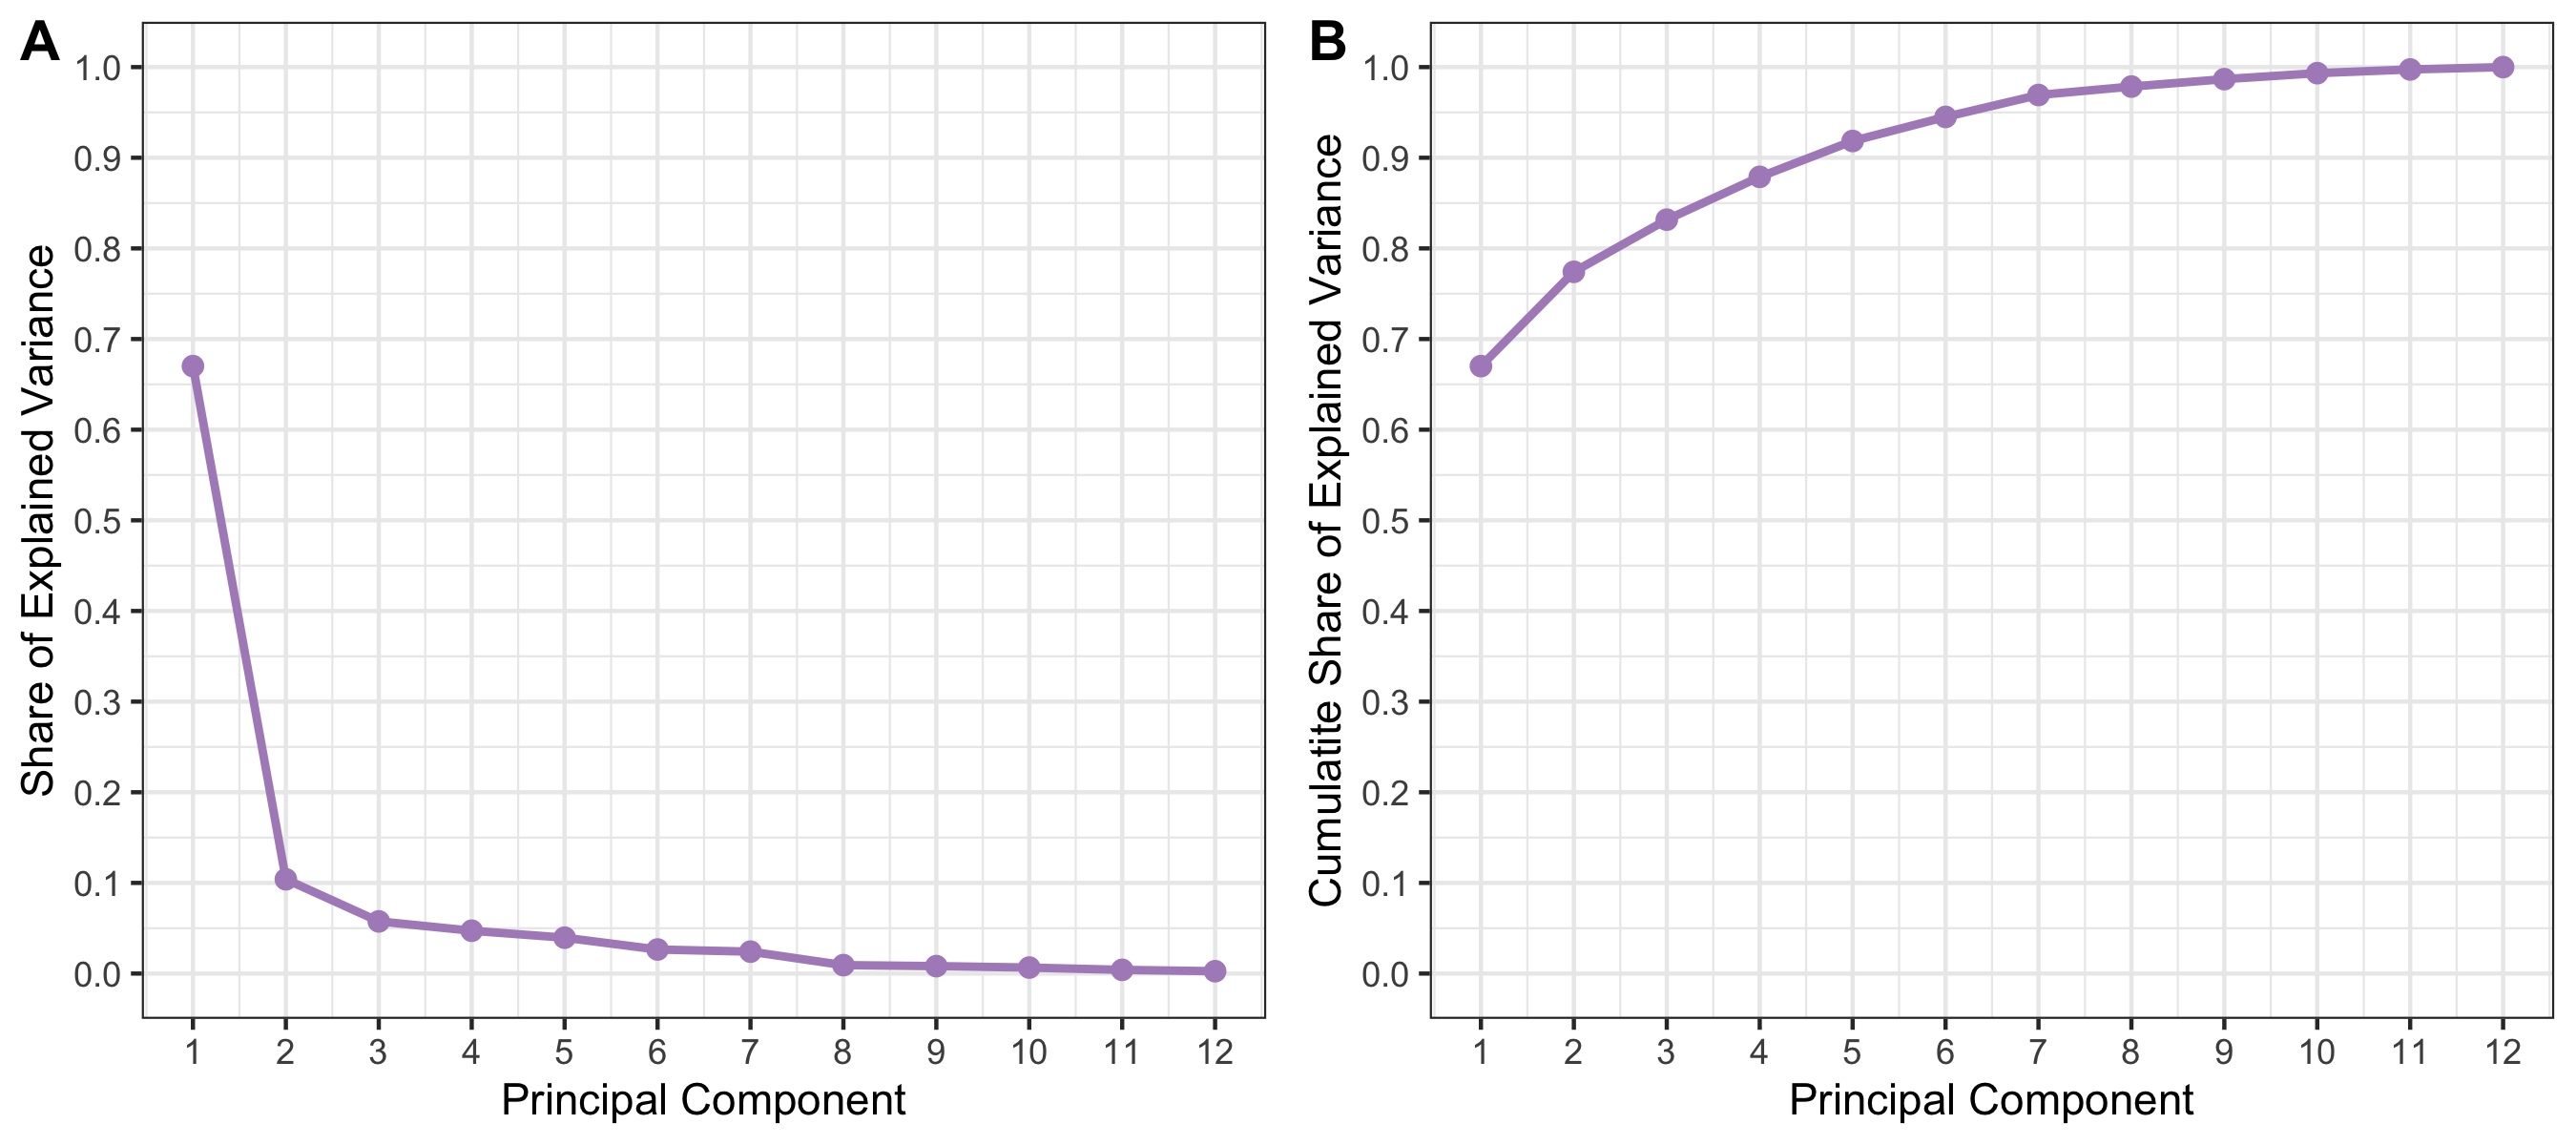
\includegraphics[scale=.15]{figures/plot_S1_LSC2_english}
 \end{figure}
\end{frame}
%----------------------------------------------------------------------%
\begin{frame}
\frametitle{Selection of factors}
\framesubtitle{Kaiser criterion}
\begin{itemize}
\item Let the columns of X be standardized, so that each variable has unit variance. 
\item In this case:

\begin{align}
trace(S) =  \sum_{j=1}^K V(F_j) = K
\end{align}

\item and recall $\sum_{j=1}^K \lambda_j= \sum_{j=1}^K V(F_j)$ then

\begin{align}
 \sum_{j=1}^K \lambda_j = K
\end{align}

\item On average, each factor contributes one unit. When $\lambda_j>1$, that factor it explains the total variance more than the average. $\rightarrow$ Retain the factors with $\lambda_j > 1$ 

\end{itemize}



\end{frame}
%----------------------------------------------------------------------%
\begin{frame}
\frametitle{Selection of factors}
\framesubtitle{Proportion of variance explained}

\begin{itemize}
\item Another approach often used in practice is to impose a threshold a priori and choose the main components based on it. 
\medskip
  \begin{itemize}
    \item For example, we could define a threshold of 90\%, which in the previous example plot would result in 5 main components. 
    \medskip
    \item Whereas if it were 70\% we would have 2 main components.
  \end{itemize}
\medskip  
\item The threshold to be defined will depend on the application, the context, and the data set. Thresholds between 70\% and 90\% are typically used.
\end{itemize}


\end{frame}
%----------------------------------------------------------------------%
\subsection{PC Computation}
%----------------------------------------------------------------------%
\begin{frame}[fragile]
\frametitle{PC Computation}

\begin{itemize}

\item Befroe I mentioned that  data was standardized, that is, re-centered to have zero mean and scaled to have variance one. 
\medskip
\item From a strictly mathematical point of view, there is nothing inherently wrong with making linear combinations of variables with different units of measurement. 
\medskip
\item However, when we use PCA we seek to maximize variance and the variance is affected by the units of measurement. 
\medskip
\item This implies that the principal components based on the covariance matrix $ S $ will change if the units of measure of one or more variables change. 


\end{itemize}


\end{frame}
%----------------------------------------------------------------------%
\begin{frame}[fragile]
\frametitle{PC Computation}

\begin{itemize}
  \item To prevent this from happening, it is common practice to standardize the variables. That is, each $ X $ value is re-centered and divided by the standard deviation:
  \medskip
    \begin{align}
      z_{ij}=\frac{x_{ij}-\bar{x_j}}{s_j}
    \end{align}
  \medskip
  \item  where $\bar{x_j}$ is the mean and ${s_j}$ is the standard deviation of column $j$. 
  \medskip
  \item Then the initial data matrix $ X $ is replaced by the standardized data matrix $ Z $.
  \medskip
  \item Note also that when standardizing the data matrix, the covariance matrix $ S $ is simply the original data correlation matrix. This is sometimes referred to in the literature as the PCA correlation matrix.
\end{itemize}

\end{frame}
%----------------------------------------------------------------------%
\begin{frame}[fragile]
\frametitle{PC Computation}
\framesubtitle{Uniqueness of the main components}

\begin{itemize}
  \item It is necessary to warn that the "loadings" of the main components $\delta$ are unique except for a sign change. 
  \medskip
  \item This implies that depending on the implementation we can obtain different results in two libraries. 
  \medskip
  \item The "loadings" will be the same but the signs may differ. 
  \medskip
  \item The signs may differ because each weight specifies a direction in k-dimensional space and the change of sign has no effect on the direction.
\end{itemize}

\end{frame}
%----------------------------------------------------------------------%
\begin{frame}[fragile]
\frametitle{PC Computation}


\begin{itemize}


  \item As a practical aside, note that \texttt{prcomp} converts $ X $ here from sparse to dense matrix storage.
  \medskip
  \item For really big text DTMs, which will be very sparse, this will cause you to run out of memory. 
\medskip
  \item A big data strategy for PCA is to first calculate the covariance matrix for $ X $ and then obtain PC rotations as the eigenvalues of this covariance matrix. 
  \medskip
    \begin{itemize}

        \item The first step can be done using sparse matrix algebra. 
        \medskip
        \item The rotations are then available as

        \begin{verbatim}
        ## eigen( xvar, symmetric = TRUE)$vec. 
        \end{verbatim}
    \end{itemize}
    \medskip
  \item There are also approximate PCA algorithms available for fast factorization on big data. See, for example, the \texttt{irlba} package for R. 
  \end{itemize}
\end{frame}

%----------------------------------------------------------------------%
\section{Factor Interpretation}
%----------------------------------------------------------------------%
\begin{frame}
\frametitle{Factor Interpretation}

\begin{itemize}
\item $f_s = X\delta'_s$ : 'loadings' often suggest that a factor works as a 'index' of a group of variables.
\bigskip
\item Idea: look at the 'loadings'
\bigskip
\item Caution: factors via principal components are orthogonal recursively.
\end{itemize}


\end{frame}


%----------------------------------------------------------------------%
\begin{frame}[fragile]
\frametitle{Factor Interpretation: Example}


\begin{itemize}
\item {\bf Congress and \theme Roll Call Voting}
\bigskip
\begin{itemize}
  \item Votes in which names and positions are recorded are called `roll calls'.
  \medskip
  \item The site {\tt voteview.com} archives vote records and the R package { \tt pscl} has tools for this data.
  \medskip
  \item 445 members in the last US House  (the $111^{th}$)
  \medskip
  \item 1647 votes:  \theme nea = -1, \nv yea=+1, \gr missing = 0.
  \medskip
  \item This leads to a large matrix of observations that can probably be reduced to simple factors {\gr (party)}.
\end{itemize}
\end{itemize}





\end{frame}


%----------------------------------------------------------------------%
\begin{frame}[fragile]
\frametitle{Factor Interpretation}

\begin{itemize}

  \item Vote components in the $\bs{111^{th}}$ house
 
 \item Each PC is $f_s = X\delta'_s$ 

  \begin{figure}[H] \centering
            \captionsetup{justification=centering}
              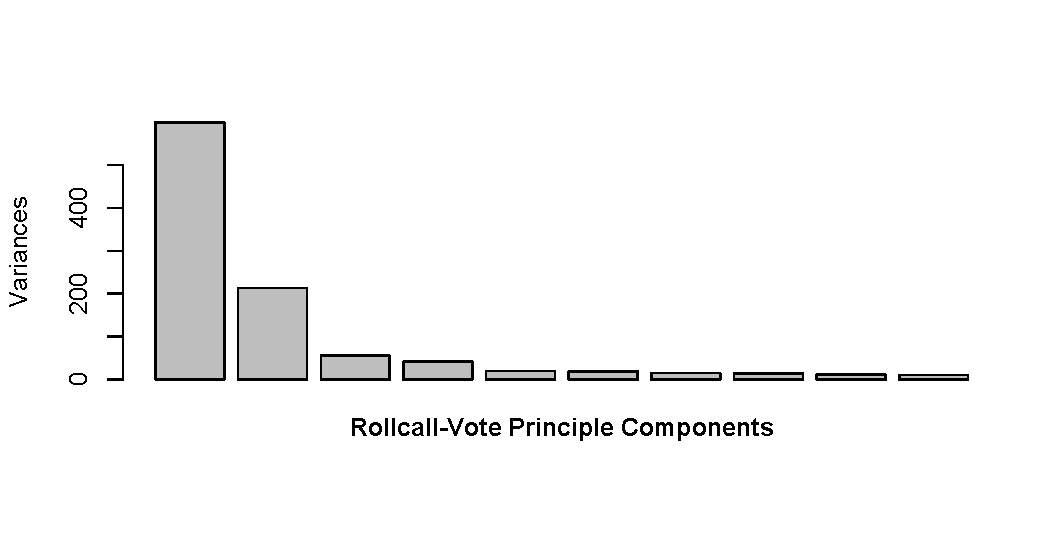
\includegraphics[scale=0.5]{figures/VOTEscree}
              
 \end{figure}

\item Huge drop in variance from $1^{st}$ to $2^{nd}$ and  $2^{nd}$ to $3^{rd}$ PC.
\item Poli-Sci holds that PC1 is usually enough to explain congress. \\\sg 2nd component has been important twice: 1860's and 1960's.

\end{itemize}


\end{frame}

%----------------------------------------------------------------------%
\begin{frame}[fragile]
\frametitle{Factor Interpretation}



\begin{itemize}

  \item Vote components in the $\bs{111^{th}}$ house
 
 \item Each PC is $F_s = X\delta_s$ 

  \begin{figure}[H] \centering
            \captionsetup{justification=centering}
              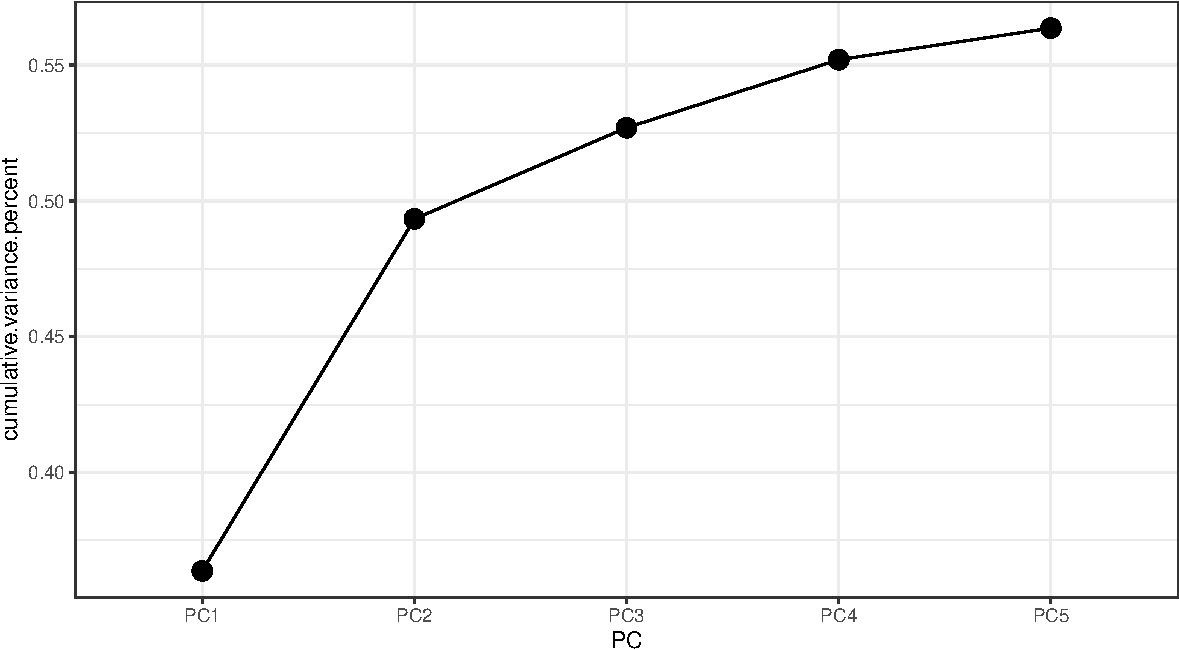
\includegraphics[scale=0.4]{figures/scree_plot}
              
 \end{figure}

\item Huge drop in variance from $1^{st}$ to $2^{nd}$ and  $2^{nd}$ to $3^{rd}$ PC.
\item Poli-Sci holds that PC1 is usually enough to explain congress. \\\sg 2nd component has been important twice: 1860's and 1960's.

\end{itemize}

\end{frame}

%----------------------------------------------------------------------%
\begin{frame}[fragile]
\frametitle{Factor Interpretation}

\begin{itemize}
\item Top two PC directions in the $\bs{111^{th}}$ house



  \begin{figure}[H] \centering
            \captionsetup{justification=centering}
              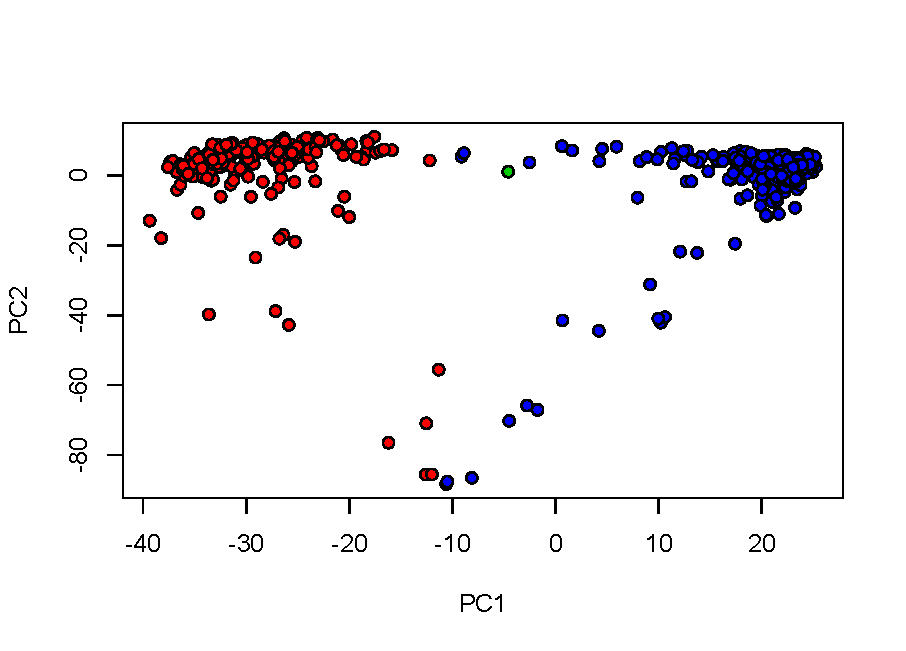
\includegraphics[scale=.5]{figures/VOTEpc}
 \end{figure}




  \item Republicans in red and Democrats in blue: 
  \begin{itemize}
  \item Clear separation on the first principal component.
  \item The second component looks orthogonal to party.
  \end{itemize}
\end{itemize}


\end{frame}


%----------------------------------------------------------------------%
\begin{frame}[fragile]
\frametitle{Factor Interpretation}




{\scriptsize \nv

{\theme \tt \#\# Far right (very conservative) \vspace{-.25cm}}
\begin{verbatim}
> sort(votepc[,1])
     BROUN (R GA-10)       FLAKE (R AZ-6)   HENSARLIN (R TX-5) 
         -39.3739409          -38.2506713          -37.5870597 
\end{verbatim}

{\theme \tt \#\# Far left (very liberal) \vspace{-.25cm}}
\begin{verbatim}
> sort(votepc[,1], decreasing=TRUE)
    EDWARDS (D MD-4)   PRICE (D NC-4)    MATSUI (D CA-5)      
         25.2915083        25.1591151         25.1248117     
\end{verbatim}       
  

{\theme \tt \#\# social issues? immigration? no clear pattern\vspace{-.25cm}}
\begin{verbatim}
> sort(votepc[,2])
     SOLIS (D CA-32) GILLIBRAND (D NY-20)      PELOSI (D CA-8) 
        -88.31350926         -87.58871687         -86.53585568 
   STUTZMAN (R IN-3)       REED (R NY-29)      GRAVES (R GA-9) 
        -85.59217310         -85.53636319         -76.49658108 
\end{verbatim}
}

\begin{itemize}
  \item PC1 is easy to read, PC2 is ambiguous (is it even meaningful?)
\end{itemize}


\end{frame}

%----------------------------------------------------------------------%
\begin{frame}[fragile]
\frametitle{Factor Interpretation}

\begin{itemize}
  \item {\bf \nv High PC1-loading votes are \theme  ideological battles.} 
  \item These tend to have  informative voting across party lines.


 \begin{figure}[H] \centering
            \captionsetup{justification=centering}
              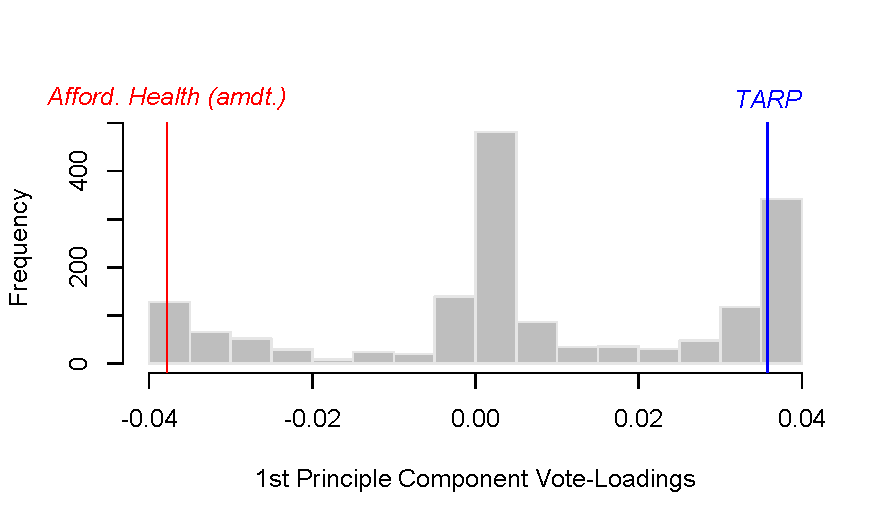
\includegraphics[scale=.5]{figures/VOTEloads}
 \end{figure}


 \footnotesize 
\item A vote for Repulican amendments to `Affordable Health Care for America' strongly indicates a negative PC1 (more conservative), while \\a vote for Troubled Asset Relief Program (TARP) indicates a positive PC1 (more progressive).
\end{itemize}

\end{frame}

%----------------------------------------------------------------------%
\begin{frame}[fragile]
\frametitle{Factor Interpretation}

\begin{itemize}
\item Look at the largest loadings in $\delta_{2}$ to discern an interpretation.



{\nv \scriptsize 
\begin{verbatim}
  > loadings[order(abs(loadings[,2]), decreasing=TRUE)[1:5],2]
   Vote.1146   Vote.658  Vote.1090  Vote.1104  Vote.1149 
  0.05605862 0.05461947 0.05300806 0.05168382 0.05155729 
\end{verbatim} }
  
\vskip -.25cm
\item These votes all correspond to near-unanimous  symbolic action.

\vskip .25cm
\bk
\item For example, 429 legislators voted for resolution 1146: \\
`{\sg Supporting the goals and ideals of a Cold War Veterans Day}'\\
{\gr If you didn't vote for this, you weren't in the house.}


 \item {{\theme Mystery Solved: } the second PC is just attendance!}
\vspace{- .1cm}
{\nv \scriptsize 
\begin{verbatim}
 > sort(rowSums(votes==0), decreasing=TRUE)
      SOLIS (D CA-32) GILLIBRAND (D NY-20)       REED (R NY-29) 
                 1628                 1619                 1562 
    STUTZMAN (R IN-3)      PELOSI (D CA-8)      GRAVES (R GA-9) 
                 1557                 1541                 1340 
\end{verbatim}}
\vspace{- .25cm}
\end{itemize}

\end{frame}
%----------------------------------------------------------------------%
\begin{frame}[fragile]
\frametitle{Principal Component Regression}


\begin{itemize}




\item The concept is very simple: instead of regressing onto $X$, use a lower dimension set of principal components $f_s$ as covariates.

\medskip
\item This works well for a few reasons:
\begin{itemize}
\item PCA reduces dimension, which is always good.
\item Higher variance covariates are good in regression, and we choose
  the top PCs to have highest variance.
\item The PCs are independent: no multicollinearity.
\end{itemize}


\item The 2-stage algorithm is straightforward. For example,

{\nv 
\begin{semiverbatim}\vspace{.25cm}\small
         mypca = prcomp(X, scale=TRUE)
         z = predict(mypca)[,1:K]
         reg = glm(y~., data=as.data.frame(z))
\end{semiverbatim}
}

\end{itemize}


\end{frame}

%----------------------------------------------------------------------%
\section{Review
 \& Next Steps}
%----------------------------------------------------------------------%
\begin{frame}
\frametitle{Review \& Next Steps}
  
\begin{itemize} 
  
  \item Factor Models
  \medskip
  \item PCA Theory
  \medskip
  \item PC Computation 
  \medskip
  \item Factor Interpretation
      \bigskip  
    \item  Next class:  More on PC regression and LDA


  \bigskip  
  \item Questions? Questions about software? 

\end{itemize}
\end{frame}
%----------------------------------------------------------------------%
\section{Further Readings}
%----------------------------------------------------------------------%
\begin{frame}
\frametitle{Further Readings}

\begin{itemize}
  
  
  \item Ahumada, H. A., Gabrielli, M. F., Herrera Gomez, M. H., \& Sosa Escudero, W. (2018). Una nueva econometría: Automatización, big data, econometría espacial y estructural.
  \medskip
  \item  Deisenroth, M. P., Faisal, A. A., \& Ong, C. S. (2020). Mathematics for machine learning. Cambridge University Press.
  \medskip
  \item James, G., Witten, D., Hastie, T., \& Tibshirani, R. (2013). An introduction to statistical learning (Vol. 112, p. 18). New York: springer.
  \medskip
  \item Murphy, K. P. (2012). Machine learning: a probabilistic perspective.    MIT press.
  \medskip
  \item Taddy, M. (2019). Business data science: Combining machine learning and economics to optimize, automate, and accelerate business decisions. McGraw Hill Professional.
  \medskip
  \item   Peña, D. (2002). Análisis de datos multivariantes (Vol. 24). Madrid:McGraw-hill.

\end{itemize}

\end{frame}
%----------------------------------------------------------------------%
%----------------------------------------------------------------------%
\end{document}
%----------------------------------------------------------------------%
%----------------------------------------------------------------------%
